\documentclass[conference]{IEEEtran}
\IEEEoverridecommandlockouts
\usepackage{cite}
\usepackage{balance}
\usepackage{amsmath,amssymb,amsfonts}
\usepackage{graphicx}
\usepackage{textcomp}
\usepackage{xcolor}
\usepackage{booktabs}
\usepackage{algorithm}
\usepackage{algorithmic}
\usepackage{tikz}
\usetikzlibrary{positioning,arrows.meta,fit,calc}
\usepackage[hidelinks]{hyperref}
\input{nums.tex}

\begin{document}

\title{Verifier-Gated Tool Use: An Agentic Re-Planning\\
Loop with a QAOA Solver for Flood\\
Shelter Assignment}

%<AUTHORS>
\author{
\IEEEauthorblockN{Nandhakumar T}
\IEEEauthorblockA{\textit{Department of Information Technology}\\
\textit{Sona College of Technology}\\
Salem, Tamil Nadu, India\\
nandhakumartm93@gmail.com}
\and
\IEEEauthorblockN{Balakarthikeyan B S}
\IEEEauthorblockA{\textit{Department of Artificial Intelligence and Data Science}\\
\textit{Sona College of Technology}\\
Salem, Tamil Nadu, India\\
balasan2626@gmail.com}
\and
\IEEEauthorblockN{Gowthaman J}
\IEEEauthorblockA{\textit{Department of Artificial Intelligence and Data Science}\\
\textit{Sona College of Technology}\\
Salem, Tamil Nadu, India\\
gowthamanjanadhran@gmail.com}
\and
\IEEEauthorblockN{Abhishek S}
\IEEEauthorblockA{\textit{Department of Artificial Intelligence and Data Science}\\
\textit{Sona College of Technology}\\
Salem, Tamil Nadu, India\\
abisheksengodan18@gmail.com}
}
%</AUTHORS>

\maketitle

\begin{abstract}
Agentic systems increasingly call external solvers as tools, and quantum optimizers are being proposed as one such tool. A quantum sampler returns a distribution, not a guaranteed answer, so an agent that dispatches its output directly inherits that uncertainty. We study this problem in a flood-evacuation setting. A loop of monitor, planner, solver and verifier agents re-plans the assignment of evacuation groups to shelters as roads close and shelters fill, using the Quantum Approximate Optimization Algorithm (QAOA) with a constraint-preserving XY mixer as one of its tools. Every plan is verified against the current state before dispatch, with fallbacks to a greedy rule, exhaustive search and finally a human. Over \Seeds{} five-event episodes from a flood digital twin (\NReplans{} re-plans, 12 qubits, exact statevector simulation), dispatching the most frequent QAOA sample without checking it would have sent an invalid plan in \RawInvalid\% of re-plans. With the verifier, no invalid plan was dispatched and the plan was optimal in \VerifiedOpt\% of re-plans. When a sixth event left \EscInfeasible{} of \EscEpisodes{} episodes without any feasible plan, the loop escalated every one of them to a human and never escalated a solvable case, while the unverified policy would have dispatched an invalid plan each time. A greedy rule with an exhaustive fallback reached \ClassicalOpt\% in about a millisecond, so the QAOA tool did not beat the classical one. Reusing QAOA angles from the previous event cut objective evaluations by \NfevSaving\%, and a stability term in the cost reduced how many groups were moved at each re-plan. Classical tools solve these instances exactly, so the contribution is the verification and fallback design for probabilistic tools. We claim no quantum speed-up.
\end{abstract}

\begin{IEEEkeywords}
agentic AI, tool use, runtime verification, QAOA, XY mixer, re-planning, plan stability, evacuation, digital twin
\end{IEEEkeywords}

\section{Introduction}
An agent that plans with tools is only as reliable as the weakest tool it trusts. Language-model agents now decide when to call calculators, search engines and code interpreters \cite{Yao2023,Schick2023}, and optimisation services are a natural next tool. Quantum optimisers are often proposed for this role in logistics and disaster response \cite{Abbas2024,Cadelina2024}. Their output, however, is a sample from a probability distribution. Even a well-trained Quantum Approximate Optimization Algorithm (QAOA) circuit \cite{Farhi2014} returns infeasible or suboptimal bitstrings with non-zero probability, and the probability depends on the instance.

In flood response, the plan that matters is re-made many times. A road closes, a shelter fills or fails, and the officer needs a new assignment of evacuation groups to shelters. Each re-plan should be valid for the state at that moment, should not move groups who are already travelling without reason, and should reach a human when no valid plan exists. A solver cannot see the plan in force or decide when to involve a person, so these requirements fall on the agent loop that calls it.

We design and evaluate such a loop. Our contributions are:
\begin{enumerate}
\item An agentic re-planning loop in which a monitor detects state changes, a planner builds a binary optimisation instance, a solver agent calls a portfolio of tools including QAOA, and a verifier checks every candidate plan against the current state, with a fixed fallback order that ends in human escalation (Fig.~\ref{fig:loop}).
\item A stability term that penalises reassigning groups between re-plans, and an angle memory that warm-starts QAOA from the previous event.
\item An evaluation over \Seeds{} five-event episodes from a flood digital twin that compares unverified, verified, portfolio, classical and exhaustive policies on validity, optimality, escalation, plan churn and cost.
\end{enumerate}
All QAOA results come from exact, noiseless classical simulation. We do not claim a quantum speed-up. Exhaustive search is included as the reference because it is exact and fast at this size.

\section{Related Work}
\textit{Tool-using agents.} ReAct interleaves reasoning traces with tool calls \cite{Yao2023}, and Toolformer learns when a call is worth making \cite{Schick2023}. Surveys of LLM-based agents identify tool reliability and the lack of verification as open problems \cite{WangL2024}. Our agents are deterministic programs, which lets us study the tool-handling logic in isolation from language-model behaviour. Variational quantum algorithms are themselves a hybrid loop in which a classical optimiser repeatedly calls a quantum circuit \cite{McClean2016}. Our setting wraps this inner loop in an outer, agentic one, and the two loops have different failure modes: the inner loop can fail to train, while the outer loop must cope with a trained circuit that still returns a bad sample.

\textit{Verified fallbacks.} The Simplex architecture runs an unverified high-performance controller alongside a verified safety controller and switches when the former leaves a safe envelope \cite{Sha2001}. Shielding applies the same idea to learned policies \cite{Alshiekh2018}. Our verifier plays the role of the switching logic, with the QAOA tool as the high-performance component and exhaustive search as the verified one. Runtime verification more generally checks each execution of a system against a specification as it happens, rather than proving the system correct in advance \cite{Leucker2009}. For a probabilistic solver, that is the only kind of guarantee available, because the same call can return a different answer each time.

\textit{Re-planning and stability.} In automated planning, repairing a plan rather than re-planning from scratch keeps the new plan close to the old one, which reduces disruption for whoever is executing it \cite{Fox2006}. Evacuation shelter allocation has a long history in operations research \cite{Sherali1991}. Flood-risk professionals who co-designed a digital twin asked above all for transparent provenance and ``what-if'' runs they could trust \cite{Underhill2026}. A re-planning loop driven by such a twin has to explain why a plan changed, and a stability term that leaves groups where they are unless moving them is clearly better makes those explanations shorter.

\textit{QAOA as a solver.} The quantum alternating operator ansatz uses mixers that preserve hard constraints \cite{Hadfield2019}, and XY mixers keep one-hot encodings valid \cite{WangZ2020}. Optimal QAOA angles concentrate across similar instances \cite{Brandao2018} and can be transferred between them \cite{Galda2021}, and angles at depth $p$ can be interpolated from depth $p-1$ \cite{Zhou2020}. Penalty formulations for assignment problems are described by Lucas \cite{Lucas2014}.

\section{Problem and Agents}
\subsection{Assignment Instance}
The digital twin models three population zones, nine junctions and three shelters joined by 22 roads, each with a travel time, flood index and congestion level from a fixed seed. Each episode follows the first four evacuation groups (8--22 people each). For group $g$ and shelter $s$, the cost $c_{gs}$ is the travel time in minutes plus five times the mean flood index of the best open path. A pair is forbidden if no open path exists, the shelter has failed or the group exceeds its remaining seats $R_s$. With $x_{gs}\in\{0,1\}$, the planner minimises
\begin{equation}
J(\mathbf{x})=\sum_{g,s}\big(c_{gs}+\mu\,[s\neq s^{\mathrm{prev}}_g]\big)x_{gs}
\label{eq:obj}
\end{equation}
subject to one shelter per group, no forbidden pair and $\sum_g n_g x_{gs}\le R_s$. Here $s^{\mathrm{prev}}_g$ is the shelter assigned to group $g$ by the plan in force and $\mu$ (minutes) is the stability weight. The term is linear in $\mathbf{x}$, so it adds no qubits or two-qubit gates.

For QAOA the planner writes the problem as a quadratic unconstrained binary optimisation with costs shifted by their per-group minimum, a penalty for forbidden pairs and a pairwise penalty $x_{gs}x_{hs}$ for any two groups that together exceed $R_s$. With $c'_{gs}=c_{gs}+\mu[s\neq s^{\mathrm{prev}}_g]-\min_{s'}(\cdot)$ the shifted cost, $\mathcal{F}$ the forbidden pairs and $\mathcal{O}$ the triples $(g,h,s)$ with $n_g+n_h>R_s$, the energy is
\begin{equation}
E(\mathbf{x})=\sum_{g,s}c'_{gs}x_{gs}+P\Big[\sum_{(g,s)\in\mathcal{F}}x_{gs}+\sum_{(g,h,s)\in\mathcal{O}}x_{gs}x_{hs}\Big],
\label{eq:energy}
\end{equation}
where $P=1+\sum_g\max_s c'_{gs}$ exceeds the total cost spread, so any penalised bitstring has higher energy than any unpenalised one. The one-hot constraint needs no penalty here because the mixer preserves it. The pairwise encoding can miss an overload by three groups, which is one reason the verifier re-checks every plan exactly. The solver uses a ring-XY mixer within each group, started from a product of W states, so every sample is one-hot by construction \cite{WangZ2020}. The circuit has depth $p=\Depth$, its angles are trained with COBYLA on the mean energy, and \Shots{} shots are drawn from the final state.

\subsection{Episode}
Each episode replays five events on a seeded twin: E0, the initial state; E1, road R5 closes; E2, Shelter A receives arrivals equal to half its capacity; E3, a further randomly chosen road closes; and E4, Shelter A fails. After each event the monitor compares the graph version and shelter states with those at the last plan. If nothing has changed, no re-plan is made.

\subsection{Agents and Policies}
Fig.~\ref{fig:loop} shows the loop, and Algorithm~\ref{alg:loop} gives the verified policy. Let $\sigma_t$ be the twin state after event $t$, with forbidden pairs $\mathcal{F}(\sigma_t)$ and remaining seats $R_s(\sigma_t)$. The verifier accepts a plan $\mathbf{x}$ when
\begin{multline}
V(\mathbf{x},\sigma_t)=\Big[\textstyle\sum_s x_{gs}=1\ \forall g\Big]\wedge\Big[x_{gs}=0\ \forall (g,s)\in\mathcal{F}(\sigma_t)\Big]\\
\wedge\Big[\textstyle\sum_g n_g x_{gs}\le R_s(\sigma_t)\ \forall s\Big].
\label{eq:ver}
\end{multline}
It reads the current state, not the instance the solver saw, so a plan that became invalid while the solver ran is rejected. Plan churn at event $t$ is the number of groups whose shelter changed,
\begin{equation}
C_t=\sum_g\big[s_g(\mathbf{x}_t)\neq s_g(\mathbf{x}_{t-1})\big],
\label{eq:churn}
\end{equation}
and the portfolio policy keeps $\arg\min\{J(\mathbf{x}) : \mathbf{x}\in\{\mathbf{x}_{\mathrm{QAOA}},\mathbf{x}_{\mathrm{greedy}}\},\ V(\mathbf{x},\sigma_t)\}$. We compare five policies on the same episodes:
\begin{itemize}
\item \textbf{Raw}: dispatch the most frequent QAOA sample without checking it.
\item \textbf{Verified}: take the cheapest feasible QAOA sample; fall back to greedy, then exhaustive search, then a human.
\item \textbf{Portfolio}: run verified QAOA and the greedy rule and keep the cheaper valid plan.
\item \textbf{Classical}: greedy, then exhaustive search, then a human.
\item \textbf{Oracle}: exhaustive search over all $3^G$ one-hot plans.
\end{itemize}
The greedy rule assigns the largest group first to its cheapest shelter with seats left.

\textit{Tool costs.} The three tools scale very differently. With $G$ groups and $S$ shelters, the greedy rule needs $O(GS)$ operations after sorting, exhaustive search checks $S^G$ plans, and exact statevector simulation of QAOA stores $2^{GS}$ amplitudes and applies $O(p\,GS)$ gates to them per evaluation. At $G=4$ and $S=3$ these are 12 operations, 81 plans and 4,096 amplitudes. Exhaustive search therefore remains the right verifier at this size, and simulation is the bottleneck, not the optimisation. On hardware, the circuit would need $GS$ qubits, so the loop's structure would stay the same while the solver tool changed; that is the setting in which the verifier and fallback order matter most, because exhaustive search would no longer be available as the last resort. To isolate the effect of verification, the raw, verified and portfolio policies are scored on the same QAOA draw at each event, which is computed on the instance of the verified policy.

\begin{figure}[t]
\centering
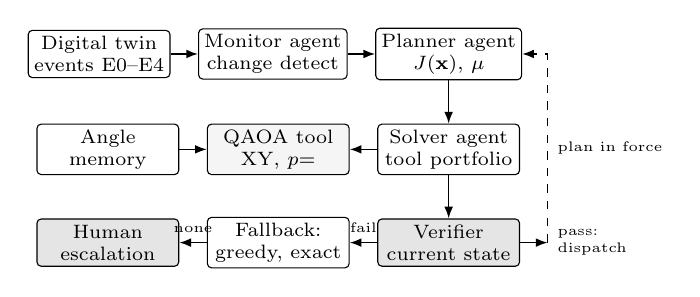
\begin{tikzpicture}[
  font=\scriptsize,
  box/.style={draw, rounded corners=1.5pt, align=center, minimum width=1.8cm, minimum height=0.6cm, inner sep=2pt},
  gate/.style={box, fill=gray!20},
  arr/.style={-{Latex[length=1.5mm]}, semithick}]
\node[box] (tw) {Digital twin\\events E0--E4};
\node[box, right=0.35cm of tw] (mon) {Monitor agent\\change detect};
\node[box, right=0.35cm of mon] (plan) {Planner agent\\$J(\mathbf{x})$, $\mu$};
\node[box, below=0.55cm of plan] (solv) {Solver agent\\tool portfolio};
\node[box, left=0.35cm of solv, fill=gray!8] (qa) {QAOA tool\\XY, $p$=\Depth};
\node[box, left=0.35cm of qa] (mem) {Angle\\memory};
\node[gate, below=0.55cm of solv] (ver) {Verifier\\current state};
\node[box, left=0.35cm of ver] (fb) {Fallback:\\greedy, exact};
\node[gate, left=0.35cm of fb] (hum) {Human\\escalation};
\draw[arr] (tw) -- (mon);
\draw[arr] (mon) -- (plan);
\draw[arr] (plan) -- (solv);
\draw[arr] (solv) -- (qa);
\draw[arr] (mem) -- (qa);
\draw[arr] (solv) -- (ver);
\draw[arr] (ver) -- node[above, font=\tiny]{fail} (fb);
\draw[arr] (fb) -- node[above, font=\tiny]{none} (hum);
\draw[arr] (ver.east) -- ++(0.35,0) node[right, align=left, font=\tiny]{pass:\\dispatch};
\draw[arr, dashed] (ver.east) ++(0.35,0) |- (plan.east) node[pos=0.25, right, font=\tiny]{plan in force};
\end{tikzpicture}
\caption{Agentic re-planning loop. Shaded blocks decide whether a plan may be dispatched. The plan in force feeds the stability term of the next re-plan, and the angle memory warm-starts the QAOA tool.}
\label{fig:loop}
\end{figure}

\begin{algorithm}[t]
\caption{Verified re-planning at one event}
\label{alg:loop}
\begin{algorithmic}[1]
\small
\IF{state key unchanged since last plan}
\STATE \textbf{return} plan in force
\ENDIF
\STATE build $J$ from the current state and plan in force
\STATE $\boldsymbol\theta\leftarrow$ memory, or INTERP training from $p=1$
\STATE draw \Shots{} shots; $\mathbf{x}\leftarrow$ cheapest one-hot sample passing the verifier
\STATE \textbf{if} none \textbf{then} $\mathbf{x}\leftarrow$ greedy; \textbf{if} it fails, $\mathbf{x}\leftarrow$ exhaustive
\IF{$\mathbf{x}$ passes the verifier}
\STATE dispatch $\mathbf{x}$; store $\mathbf{x}$ and $\boldsymbol\theta$
\ELSE
\STATE escalate to a human with the failed checks
\ENDIF
\end{algorithmic}
\end{algorithm}

\section{Experimental Setup}
We ran \Seeds{} episodes with twin seeds $42+17i$, $i=0,\dots,\SeedsLast$, giving \NEvents{} events. Every event changed the state, so the monitor triggered a re-plan at all \NReplans{} events. At least one feasible plan existed at every event, so the escalation branch of the loop was not reached in these episodes. To test it, we extended each episode with a sixth event, E5, in which Shelter B also fails and only Shelter C remains, and ran the verified policy with angle memory through all six events. Each QAOA call was simulated as an exact $2^{12}$-amplitude statevector. In the baseline configuration ($\mu=0$, cold start), each call trained depths 1 to \Depth{} with INTERP initialisation \cite{Zhou2020} and two random restarts per depth. With angle memory, a call started a single optimisation from the angles stored at the previous event. We also ran the verified and oracle policies with $\mu=3$ and $\mu=6$ minutes, with memory on. Times are wall-clock on a consumer laptop and include simulation, so they describe this prototype, not a quantum device.

\section{Results}
\subsection{Verification and Fallback}
Table~\ref{tab:policy} summarises the baseline configuration. Dispatching the most frequent QAOA sample without checking would have sent an invalid plan in \RawInvalid\% of re-plans. The XY mixer guarantees one-hot samples, so these failures were capacity and forbidden-pair violations. They were concentrated in the events that made capacity tight (Table~\ref{tab:event}). The verified policy dispatched no invalid plan and reached the exhaustive optimum in \VerifiedOpt\% of re-plans, with a mean excess cost of \VerifiedGap~min. In \VerifiedFallback\% of re-plans none of the \Shots{} shots was feasible and the greedy fallback supplied the plan.

The portfolio policy reached \PortfolioOpt\% optimal plans; the greedy rule supplied the kept plan in \PortfolioGreedyWon\% of re-plans. The classical policy reached \ClassicalOpt\%, more than verified QAOA, at a fraction of the time. Its mean time per re-plan was \ClassicalMs~ms, against \VerifiedMs~ms of simulated training and sampling for the verified QAOA policy.

\begin{table}[t]
\caption{Re-planning policies, \NReplans{} re-plans ($\mu=0$, cold start)}
\label{tab:policy}
\centering
\footnotesize
\setlength{\tabcolsep}{2.4pt}
\begin{tabular}{lccccc}
\toprule
Policy & Invalid (\%) & Esc. & Opt. (\%) & Gap (min) & ms\\
\midrule
\input{tab_policy.tex}
\bottomrule
\multicolumn{6}{l}{\scriptsize Invalid = dispatched plan violating a constraint. Opt. and Gap over feasible re-plans.}\\
\end{tabular}
\end{table}

\begin{table}[t]
\caption{Re-plans, infeasible events and unverified failures by event}
\label{tab:event}
\centering
\setlength{\tabcolsep}{5pt}
\begin{tabular}{lccc}
\toprule
Event & Re-plans & No feasible plan & Raw invalid\\
\midrule
\input{tab_event.tex}
\bottomrule
\end{tabular}
\end{table}

Table~\ref{tab:evopt} breaks the cold configuration down by event. All \FallbackTotal{} fallbacks happened after E1, when the surge, the extra closure or the shelter failure had removed many plans from the feasible set. With $N$ independent shots and a feasibility probability $P_{\mathrm{feas}}$, the chance that no shot is feasible is
\begin{equation}
P_{\mathrm{fb}}=(1-P_{\mathrm{feas}})^{N},
\label{eq:fb}
\end{equation}
which is negligible for $N=\Shots$ unless $P_{\mathrm{feas}}$ falls to a few percent. The observed fallbacks therefore point to events where the trained state put almost no weight on feasible plans, not to an unlucky draw.

\begin{table}[t]
\caption{Optimal plans (\%) and fallbacks by event ($\mu=0$, cold start, 30 episodes)}
\label{tab:evopt}
\centering
\footnotesize
\setlength{\tabcolsep}{3pt}
\begin{tabular}{lccccc}
\toprule
Event & Raw & Verified & Portfolio & Classical & Fallbacks\\
\midrule
\input{tab_evopt.tex}
\bottomrule
\multicolumn{6}{l}{\scriptsize Raw counts only valid plans as optimal; an invalid raw plan is never optimal.}\\
\end{tabular}
\end{table}

\subsection{Escalation}
With Shelter B failed as well as Shelter A, the remaining shelter could not take all four groups in \EscInfeasible{} of the \EscEpisodes{} episodes. In each of these the QAOA tool returned no feasible sample, the greedy fallback failed and exhaustive search confirmed that no plan existed, so the loop escalated to a human with the list of failed checks. There were \EscWrong{} wrong escalations, cases escalated although a valid plan existed, and \EscMissed{} missed ones. The raw policy, which dispatches the most frequent sample, would have sent an invalid plan in all \EscRawInvalid{} infeasible cases, since it has no way to recognise that no valid plan exists. This is the situation in which an unverified tool is most dangerous: every answer it can give is wrong, and it still gives one.

\subsection{Angle Memory}
Starting each QAOA call from the previous event's angles reduced the mean number of objective evaluations from \ColdNfev{} to \WarmNfev{} (\NfevSaving\% fewer) and the mean time per verified re-plan from \ColdMs{} to \WarmMs~ms. The verified policy reached the optimum in \WarmOpt\% of feasible re-plans with memory, against \ColdOpt\% without. Consecutive events change only a few costs and capacities, so the optimal angles move little. This agrees with reports that QAOA angles concentrate across similar instances \cite{Brandao2018,Galda2021}. Fig.~\ref{fig:nfev} shows where the saving came from. With memory, the first re-plan of each episode (E0) still paid the full cost of depth-progressive training, \NfevEzeroWarm{} evaluations on average, and every later event needed only \NfevLaterWarm{}. In a long incident with many re-plans, the cost per re-plan would approach the later figure.

\begin{figure}[t]
\centering
\includegraphics[width=\columnwidth]{fig_nfev.pdf}
\caption{Mean QAOA objective evaluations per re-plan by event, without and with angle memory ($\mu=0$).}
\label{fig:nfev}
\end{figure}

\subsection{Robustness Across Configurations}
Table~\ref{tab:cfg} repeats the main comparison in all four configurations. The verified and portfolio policies dispatched no invalid plan in any of them. The share of invalid plans that the raw policy would have dispatched fell from \RawInvalid\% with cold starts to \RawInvWarm\% with angle memory and \RawInvMuSix\% with $\mu=6$, We did not isolate the cause. A plausible reason is that warm-started angles are already tuned to a closely related instance and that the stability term raises the energy of plans that move groups, so both concentrate probability on plans near one that was valid a moment ago. The raw policy is still unsafe in every configuration. Fig.~\ref{fig:event} shows that its failures occurred only after the shelter surge, the extra closure and the shelter failure: \RawInvEtwo, \RawInvEthree{} and \RawInvEfour{} of 30 episodes in the cold configuration, and none at E0 or E1 in any configuration. These are the events where the cheapest-looking plan overloads a shelter.

\begin{table}[t]
\caption{Policies across configurations (\NReplans{} re-plans each)}
\label{tab:cfg}
\centering
\footnotesize
\setlength{\tabcolsep}{2.6pt}
\begin{tabular}{ccccccc}
\toprule
$\mu$ & angles & Raw invalid & Ver. opt. & Port. opt. & Class. opt. & Evals\\
\midrule
\input{tab_cfg.tex}
\bottomrule
\multicolumn{7}{l}{\scriptsize All values in \%, except Evals = mean QAOA objective evaluations per re-plan.}\\
\end{tabular}
\end{table}

\begin{figure}[t]
\centering
\includegraphics[width=\columnwidth]{fig_event.pdf}
\caption{Episodes (out of 30) in which the most frequent QAOA sample would have been an invalid plan, by event and configuration.}
\label{fig:event}
\end{figure}

\subsection{Plan Stability}
Table~\ref{tab:mu} and Fig.~\ref{fig:trade} show the effect of the stability weight. For the exhaustive planner, raising $\mu$ from 0 to 6 minutes changed the mean number of groups reassigned per re-plan from \OracleChurnMuZero{} to \OracleChurnMuSix{}, while the mean travel cost of the dispatched plan changed from \OracleTravelMuZero{} to \OracleTravelMuSix~min. The verified QAOA policy followed the same direction. Without the stability term it reassigned \VerChurnCold{} groups per re-plan, against \OracleChurnCold{} for exhaustive search, because QAOA samples choose among plans of nearly equal cost at random. A small $\mu$ breaks these ties in favour of the plan in force, and at $\mu=6$ the verified policy reached the optimum of (\ref{eq:obj}) in \VerOptMuSix\% of re-plans. A small $\mu$ removes reassignments between plans of nearly equal cost, which an officer would otherwise have to communicate to teams already on the road.

\begin{table}[t]
\caption{Stability weight $\mu$ (minutes), with angle memory}
\label{tab:mu}
\centering
\setlength{\tabcolsep}{4pt}
\begin{tabular}{ccccc}
\toprule
 & \multicolumn{2}{c}{QAOA + verifier} & \multicolumn{2}{c}{Exhaustive}\\
$\mu$ & churn & cost (min) & churn & cost (min)\\
\midrule
\input{tab_mu.tex}
\bottomrule
\multicolumn{5}{l}{\scriptsize churn = groups reassigned per re-plan after E0;}\\
\multicolumn{5}{l}{\scriptsize cost = mean travel cost of dispatched plans.}\\
\end{tabular}
\end{table}

\begin{figure}[t]
\centering
\includegraphics[width=\columnwidth]{fig_tradeoff.pdf}
\caption{Plan churn against travel cost for three stability weights.}
\label{fig:trade}
\end{figure}

\textit{Reproducibility.} The episodes, events and QAOA draws are fixed by the seeds above, and the simulator, the agent loop and the tables are generated by scripts in the prototype repository. Wall-clock times are the only values that change between runs.

\section{Discussion and Limitations}
The verifier did the work that made the QAOA tool usable. Without it, a solver that was right most of the time still produced invalid dispatches, and these failures clustered in the events where capacity was tight, which are the events that matter most. With it, the loop never dispatched an invalid plan. In the extended episodes it handed every infeasible situation to a human, and it never escalated a situation that had a valid plan. The same structure applies to any probabilistic tool, whether a quantum sampler, a heuristic or a learned policy. We draw four design rules from the experiments. First, verify against the state at dispatch time, not the state the tool saw. Second, prefer the best verified sample to the most frequent sample, since the most frequent sample was invalid in up to a fifth of re-plans. Third, run a cheap classical tool in parallel and keep the better valid plan, which raised optimality at no risk. Fourth, carry tool state such as QAOA angles across events, because consecutive re-planning problems are similar and the saving in evaluations was large.

Latency also matters in practice. The verified QAOA policy needed seconds of simulated training per re-plan, and a hardware run would add queueing and many circuit executions per evaluation. An evacuation plan needed within a minute could not wait for such a tool without a classical plan already in hand. The portfolio design handles this: the greedy plan is available immediately and the QAOA plan replaces it only if it arrives in time and is better.

The results do not support using QAOA on these instances in practice. Exhaustive search over 81 plans is exact and takes milliseconds, and the greedy rule is nearly as good. The QAOA tool earns its place in the loop only as a stand-in for future solvers on instances too large to enumerate, and our experiments say nothing about how it would perform on hardware or at that scale.

Several threats to validity apply. The raw, verified and portfolio policies share one draw per event, so their differences come from the selection rule alone, but the run-to-run variance of a single draw is not measured. The greedy rule and exhaustive search are deterministic and see the same instances, which favours them in a comparison of optimality. The optimality figures are relative to (\ref{eq:obj}) with the current $\mu$, so a plan that is optimal at $\mu=6$ can cost more travel time than the $\mu=0$ optimum. Further limits apply. All circuits were noiseless simulations at 12 qubits. Each episode follows one fixed sequence of events on a small synthetic network, and accessibility never constrained the plan because every shelter is accessible. The stability weight is a single scalar that treats all reassignments as equal, whereas moving a group already on the road costs more than moving one that has not left. The raw, verified and portfolio policies shared one QAOA draw per event, which makes them directly comparable but does not show the variance between draws. Escalation was tested with one kind of infeasibility, a double shelter failure, and no officer took part in the evaluation.

\section{Conclusion}
We built an agentic loop that uses QAOA as one tool among several for re-planning flood shelter assignments, and placed a verifier and a fixed fallback order between the tool and dispatch. On \Seeds{} digital-twin episodes, unverified QAOA output would have produced invalid plans in \RawInvalid\% of re-plans. The verified loop produced none, escalated all \EscInfeasible{} infeasible situations created by a double shelter failure, and never escalated a solvable one, although a greedy rule reached the optimum more often than QAOA at a tiny fraction of the cost. Angle memory and a stability term made re-planning cheaper and less disruptive. For agent design, the results mean that a probabilistic tool needs a verifier that checks its output against the current state, a fallback, and a route to a human. They make no case for quantum advantage.

\section*{Acknowledgment}
The authors thank the OpenStreetMap contributors and Open-Meteo for openly available data used by the digital twin.
In line with the IEEE policy on AI-generated content, the authors disclose that Claude (Anthropic) was used to help edit and restructure the text of all sections and to draft the simulation, experiment and plotting scripts. All experiments use the authors' own software and can be reproduced with fixed seeds. The authors checked every number, claim and reference and take full responsibility for the content.

\balance
\begin{thebibliography}{00}
\bibitem{Yao2023} S. Yao \textit{et al.}, ``ReAct: Synergizing reasoning and acting in language models,'' in \textit{Proc. Int. Conf. Learn. Represent. (ICLR)}, 2023.
\bibitem{Schick2023} T. Schick \textit{et al.}, ``Toolformer: Language models can teach themselves to use tools,'' in \textit{Adv. Neural Inf. Process. Syst. 36}, 2023, pp. 68539--68551.
\bibitem{Abbas2024} A. Abbas \textit{et al.}, ``Challenges and opportunities in quantum optimization,'' \textit{Nat. Rev. Phys.}, vol. 6, pp. 718--735, 2024.
\bibitem{Cadelina2024} A. R. Cadeli\~{n}a \textit{et al.}, ``D-Wave implementation of quantum annealing for optimal resource allocation in disaster response operation of Marikina City,'' \textit{ECTI Trans. Comput. Inf. Technol.}, vol. 18, no. 1, pp. 24--33, 2024.
\bibitem{Farhi2014} E. Farhi, J. Goldstone, and S. Gutmann, ``A quantum approximate optimization algorithm,'' arXiv:1411.4028, 2014.
\bibitem{WangL2024} L. Wang \textit{et al.}, ``A survey on large language model based autonomous agents,'' \textit{Front. Comput. Sci.}, vol. 18, no. 6, Art. no. 186345, 2024.
\bibitem{McClean2016} J. R. McClean, J. Romero, R. Babbush, and A. Aspuru-Guzik, ``The theory of variational hybrid quantum-classical algorithms,'' \textit{New J. Phys.}, vol. 18, no. 2, Art. no. 023023, 2016.
\bibitem{Sha2001} L. Sha, ``Using simplicity to control complexity,'' \textit{IEEE Softw.}, vol. 18, no. 4, pp. 20--28, 2001.
\bibitem{Alshiekh2018} M. Alshiekh, R. Bloem, R. Ehlers, B. K\"{o}nighofer, S. Niekum, and U. Topcu, ``Safe reinforcement learning via shielding,'' in \textit{Proc. AAAI Conf. Artif. Intell.}, vol. 32, no. 1, 2018, pp. 2669--2678.
\bibitem{Leucker2009} M. Leucker and C. Schallhart, ``A brief account of runtime verification,'' \textit{J. Log. Algebr. Program.}, vol. 78, no. 5, pp. 293--303, 2009.
\bibitem{Fox2006} M. Fox, A. Gerevini, D. Long, and I. Serina, ``Plan stability: Replanning versus plan repair,'' in \textit{Proc. 16th Int. Conf. Automated Planning Scheduling (ICAPS)}, 2006, pp. 212--221.
\bibitem{Sherali1991} H. D. Sherali, T. B. Carter, and A. G. Hobeika, ``A location-allocation model and algorithm for evacuation planning under hurricane/flood conditions,'' \textit{Transp. Res. B, Methodol.}, vol. 25, no. 6, pp. 439--452, 1991.
\bibitem{Underhill2026} H. Underhill, L. McEwen, and T. Coulthard, ```That's the dream, right?': Reflections on the co-design of an environmental digital twin by flood risk management professionals,'' \textit{Front. Environ. Sci.}, vol. 13, Art. no. 1724250, 2026.
\bibitem{Hadfield2019} S. Hadfield, Z. Wang, B. O'Gorman, E. G. Rieffel, D. Venturelli, and R. Biswas, ``From the quantum approximate optimization algorithm to a quantum alternating operator ansatz,'' \textit{Algorithms}, vol. 12, no. 2, Art. no. 34, 2019.
\bibitem{WangZ2020} Z. Wang, N. C. Rubin, J. M. Dominy, and E. G. Rieffel, ``XY mixers: Analytical and numerical results for the quantum alternating operator ansatz,'' \textit{Phys. Rev. A}, vol. 101, no. 1, Art. no. 012320, 2020.
\bibitem{Brandao2018} F. G. S. L. Brand\~{a}o, M. Broughton, E. Farhi, S. Gutmann, and H. Neven, ``For fixed control parameters the quantum approximate optimization algorithm's objective function value concentrates for typical instances,'' arXiv:1812.04170, 2018.
\bibitem{Galda2021} A. Galda, X. Liu, D. Lykov, Y. Alexeev, and I. Safro, ``Transferability of optimal QAOA parameters between random graphs,'' in \textit{Proc. IEEE Int. Conf. Quantum Comput. Eng. (QCE)}, 2021, pp. 171--180.
\bibitem{Zhou2020} L. Zhou, S.-T. Wang, S. Choi, H. Pichler, and M. D. Lukin, ``Quantum approximate optimization algorithm: Performance, mechanism, and implementation on near-term devices,'' \textit{Phys. Rev. X}, vol. 10, no. 2, Art. no. 021067, 2020.
\bibitem{Lucas2014} A. Lucas, ``Ising formulations of many NP problems,'' \textit{Front. Phys.}, vol. 2, Art. no. 5, 2014.
\end{thebibliography}

\end{document}
